\documentclass[aspectratio=169,10pt]{beamer}

% ============================================================
% HUST-styled Beamer theme (built from scratch — no official
% HUST .sty/template was available to reuse; colors and the
% dotted decorative pattern are visual approximations of a
% reference HUST deck, not official brand assets. Swap
% \hustred/\hustgold or the logo placeholder below if exact
% brand values become available.)
% ============================================================
\usetheme{default}
\usepackage{fontspec}
\usepackage{tikz}
\usepackage{booktabs}
\usepackage[table]{xcolor}
\usepackage[most]{tcolorbox}
\usetikzlibrary{calc}

\definecolor{hustred}{HTML}{C8102E}
\definecolor{hustgold}{HTML}{F2A900}
\definecolor{cardgray}{HTML}{F0F0F0}
\definecolor{inkgray}{HTML}{52514E}

\setbeamertemplate{navigation symbols}{}
\setbeamersize{text margin left=0.9cm, text margin right=0.9cm}
\setbeamercolor{background canvas}{bg=white}
\setbeamercolor{normal text}{fg=black}
\setbeamerfont{normal text}{family=\sffamily}
\setbeamercolor{frametitle}{bg=hustred, fg=white}
\setbeamerfont{frametitle}{series=\bfseries, size=\Large}
\setbeamertemplate{itemize items}[circle]
\setbeamercolor{itemize item}{fg=hustred}

% ---- Custom frame title: red bar + page badge + gold rule ----
\setbeamertemplate{frametitle}{%
  \vskip-1pt%
  \makebox[0pt][l]{\hspace*{-0.9cm}%
  
\begin{tikzpicture}[baseline=0pt]
    \useasboundingbox (0,0) rectangle (\paperwidth,1.15cm);
    \fill[hustred] (0,0) rectangle (\paperwidth,1.15cm);
    \node[anchor=west, text=white, font=\bfseries\Large, align=left, text width=\paperwidth-2.6cm] at (0.5cm,0.6cm) {\insertframetitle};
    \node[anchor=east, text=white, font=\normalsize] at ($(\paperwidth,0)+(-0.5cm,0.6cm)$) {\insertframenumber/\inserttotalframenumber};
  \end{tikzpicture}}\par
  \makebox[0pt][l]{\hspace*{-0.9cm}{\color{hustgold}\rule{\paperwidth}{2.2pt}}}\par
  \vskip 0.15cm
}

% ---- Custom footline: text logo lockup + thin rule ----
\setbeamertemplate{footline}{%
  \makebox[0pt][l]{\hspace*{-0.9cm}{\color{hustred!60}\rule{\paperwidth}{0.6pt}}}\par
  \vskip 1pt
  \hspace{0.9cm}%
  \raisebox{0pt}{\tikz\node[fill=hustred, text=white, font=\bfseries\tiny, inner sep=2pt]{H};}%
  \hspace{3pt}{\tiny\color{inkgray} HUST \textbar{} Customer Churn Prediction}%
  \vskip 2pt
}

% ---- Reusable macros: numbered card, stat tile ----
\newcommand{\cardbadge}[1]{\tikz[baseline=-0.65ex]{\node[circle, fill=hustred, text=white, font=\bfseries\small, inner sep=0pt, minimum size=20pt] {#1};}}

\newcommand{\card}[3]{%
  \begin{tikzpicture}
    \node[rounded corners=6pt, fill=cardgray, inner sep=8pt, text width=3.3cm, align=left, anchor=north west] {%
      \cardbadge{#1}\\[6pt]
      {\bfseries\small\color{hustred} #2}\\[3pt]
      {\scriptsize\color{inkgray} #3}%
    };
  \end{tikzpicture}%
}

\newcommand{\stattile}[2]{%
  \begin{tikzpicture}
    \node[rounded corners=6pt, fill=cardgray, inner sep=6pt, minimum width=2.9cm, align=center] {%
      \begin{minipage}{2.5cm}\centering
        {\color{hustred}\bfseries\large #1}\\[0pt]
        {\scriptsize\color{inkgray} #2}
      \end{minipage}%
    };
  \end{tikzpicture}%
}

% ---- Decorative dot spray (TikZ, procedural — no external image) ----
% Must be called *inside* an existing tikzpicture, given a coordinate name,
% e.g. \dotspray{(mycenter)}{hustred} after \coordinate (mycenter) at (...);
\newcommand{\dotspray}[2]{%
  \foreach \r in {0.3,0.7,...,3.3}{
    \foreach \a in {0,20,...,340}{
      \pgfmathsetmacro{\op}{max(0.12,1-\r/3.6)}
      \filldraw[#2, opacity=\op] ($#1+(\a:\r)$) circle (1.3pt);
    }
  }
}


% ---- Data Understanding slides: extra helpers ----
\definecolor{cardgrayd}{HTML}{F0F0F0}
\tcbset{
  dcard/.style={enhanced, boxrule=0pt, arc=3pt, colback=cardgray,
                left=6pt, right=6pt, top=4pt, bottom=4pt,
                fontupper=\footnotesize, before upper={\raggedright}},
  ddark/.style={dcard, colback=hustred, coltext=white},
  dwarn/.style={dcard, colback=hustgold!18, borderline west={2pt}{0pt}{hustgold}},
  dfig/.style={enhanced, boxrule=0.4pt, colframe=black!12, arc=4pt,
               colback=white, left=3pt, right=3pt, top=3pt, bottom=3pt}
}
\newcommand{\dhead}[1]{{\bfseries\normalsize\color{hustred}#1}}
\newcommand{\dheadline}[1]{{\bfseries\normalsize\color{inkgray}#1}\par\vspace{1pt}}
\newcommand{\dnext}[1]{\vfill\noindent{\bfseries\scriptsize\color{hustred}#1}}

\title{Data Understanding}
\author{}
\date{}

\begin{document}

% ============================================================
% 1. Data requirement and collection
% ============================================================
\begin{frame}[t]{1 \textperiodcentered{} From transactions to behaviour and churn labels}
  \vspace*{-0.55cm}
  \begin{columns}[T]
    \begin{column}{0.33\textwidth}
      \begin{tcolorbox}[ddark, height=4.9cm]
        {\bfseries\tiny\color{hustgold}DATA SOURCE}\\[1pt]
        {\bfseries\large Online Retail II}\\[1pt]
        {\scriptsize\color{white!80}Transactions of an online retailer, Dec 2009 -- Dec 2011}\\[-1pt]
        {\color{hustgold}\rule{\linewidth}{0.8pt}}\\[3pt]
        \begin{tabular}{@{}p{0.56\linewidth}@{}p{0.42\linewidth}@{}}
          {\bfseries\normalsize 1,067,371} & {\bfseries\normalsize 53,628}\\[-2pt]
          {\tiny\color{white!80}transaction lines} & {\tiny\color{white!80}invoices}\\[4pt]
          {\bfseries\normalsize 5,942} & {\bfseries\normalsize \pounds19.3M}\\[-2pt]
          {\tiny\color{white!80}customers} & {\tiny\color{white!80}total revenue}\\[4pt]
          {\bfseries\normalsize 43} & {\bfseries\normalsize 8}\\[-2pt]
          {\tiny\color{white!80}countries, UK 91.9\%} & {\tiny\color{white!80}fields}
        \end{tabular}
      \end{tcolorbox}
    \end{column}
    \begin{column}{0.63\textwidth}
      \begin{columns}[T]
        \begin{column}{0.49\linewidth}
          \begin{tcolorbox}[dcard, height=1.95cm]
            \dhead{Customer}\\
            {\bfseries\scriptsize Customer ID, Country}\\
            {\tiny\color{inkgray}Identify customers and support segmentation.}
          \end{tcolorbox}
        \end{column}
        \begin{column}{0.49\linewidth}
          \begin{tcolorbox}[dcard, height=1.95cm]
            \dhead{Transactions}\\
            {\bfseries\scriptsize Invoice, InvoiceDate, Quantity, Price}\\
            {\scriptsize\color{inkgray}Build order history and purchase metrics.}
          \end{tcolorbox}
        \end{column}
      \end{columns}
      \vspace{2pt}
      \begin{columns}[T]
        \begin{column}{0.49\linewidth}
          \begin{tcolorbox}[dcard, height=1.95cm]
            \dhead{Products}\\
            {\bfseries\scriptsize StockCode, Description}\\
            {\scriptsize\color{inkgray}Measure product diversity and purchase patterns.}
          \end{tcolorbox}
        \end{column}
        \begin{column}{0.49\linewidth}
          \begin{tcolorbox}[dcard, height=1.95cm]
            \dhead{Time and labels}\\
            {\bfseries\scriptsize Customer ID, InvoiceDate, valid purchases}\\
            {\scriptsize\color{inkgray}Create observation windows and define churn in the prediction horizon.}
          \end{tcolorbox}
        \end{column}
      \end{columns}
      \vspace{2pt}
      \begin{tcolorbox}[dwarn]
        {\scriptsize\bfseries Limitation:} {\scriptsize no campaign or marketing-cost fields, so campaign ROI cannot be measured directly.}
      \end{tcolorbox}
    \end{column}
  \end{columns}
  \dnext{Next: how do customers buy over the year? $\rightarrow$}
  \note{Our starting question is simple: with a limited retention budget, which
  customers should we keep, and when should we act? All we have is two years of
  transactions from an online retailer: about a million lines and 5,900
  customers. There are no contracts and no marketing costs, so both value and
  churn have to be inferred from how people buy. (About 20 seconds)}
\end{frame}

% ============================================================
% 2. Trend and revenue source
% ============================================================
\begin{frame}[t]{2 \textperiodcentered{} Revenue is seasonal, and repeat customers carry it}
  \vspace*{-0.55cm}
  \begin{columns}[T]
    \begin{column}{0.47\textwidth}
      \begin{tcolorbox}[dfig]
        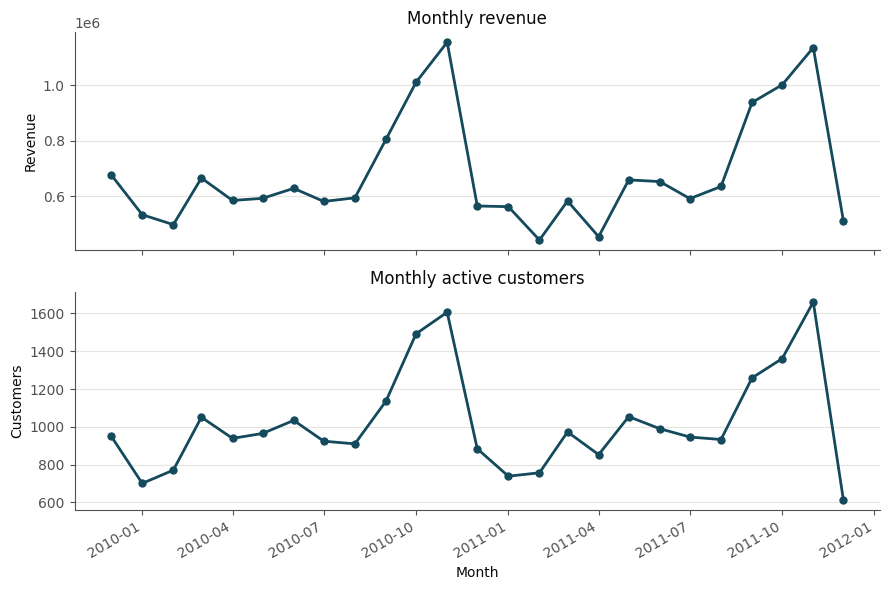
\includegraphics[width=\linewidth]{figures/monthly_revenue_customers.png}
      \end{tcolorbox}
    \end{column}
    \begin{column}{0.49\textwidth}
      \begin{tcolorbox}[dcard]
        {\bfseries\large\color{hustred}$\sim$1,040 customers/month}\\
        {\scriptsize\color{inkgray}Median revenue $\approx$ \pounds595K/month (\pounds442K -- \pounds1.16M).}
      \end{tcolorbox}
      \vspace{1pt}
      \begin{tcolorbox}[dwarn]
        {\bfseries\large\color{hustred}Peak in Oct -- Nov}\\
        {\scriptsize\color{inkgray}Nov 2010: \pounds1.16M \textperiodcentered{} Nov 2011: \pounds1.14M. Pre-Christmas ordering; December drops sharply.}
      \end{tcolorbox}
      \vspace{1pt}
      \begin{tcolorbox}[ddark]
        {\bfseries\large 72\% of customers $\rightarrow$ 97\% of revenue}\\[2pt]
        {\scriptsize Repeat buyers (72.3\%) generate 95.6\% of orders and 96.7\% of revenue.
         \textcolor{hustgold}{One-time buyers: 27.6\% of customers, 3.3\% of revenue.}}
      \end{tcolorbox}
    \end{column}
  \end{columns}
  \dnext{But in retail nobody cancels. When is a customer lost? $\rightarrow$}
  \note{Sales are seasonal, peaking before Christmas and dropping sharply in
  December. More importantly, 72\% of customers buy more than once, and they
  bring 97\% of revenue. So retention is where the value is. But in retail
  nobody cancels, so first we need to decide when a customer counts as lost.
  (About 25 seconds)}
\end{frame}

% ============================================================
% 3. Defining churn
% ============================================================
\begin{frame}[t]{3 \textperiodcentered{} Churn is inferred from purchase rhythm: $H=90$ days}
  \vspace*{-0.2cm}
  {\tiny No contracts in retail $\rightarrow$ customers never ``cancel'' $\rightarrow$
   \textcolor{hustred}{\bfseries churn = no purchase within $H$ days}}\par\vspace{3pt}
  \begin{columns}[T]
    \begin{column}{0.50\textwidth}
      \begin{tcolorbox}[dfig]
        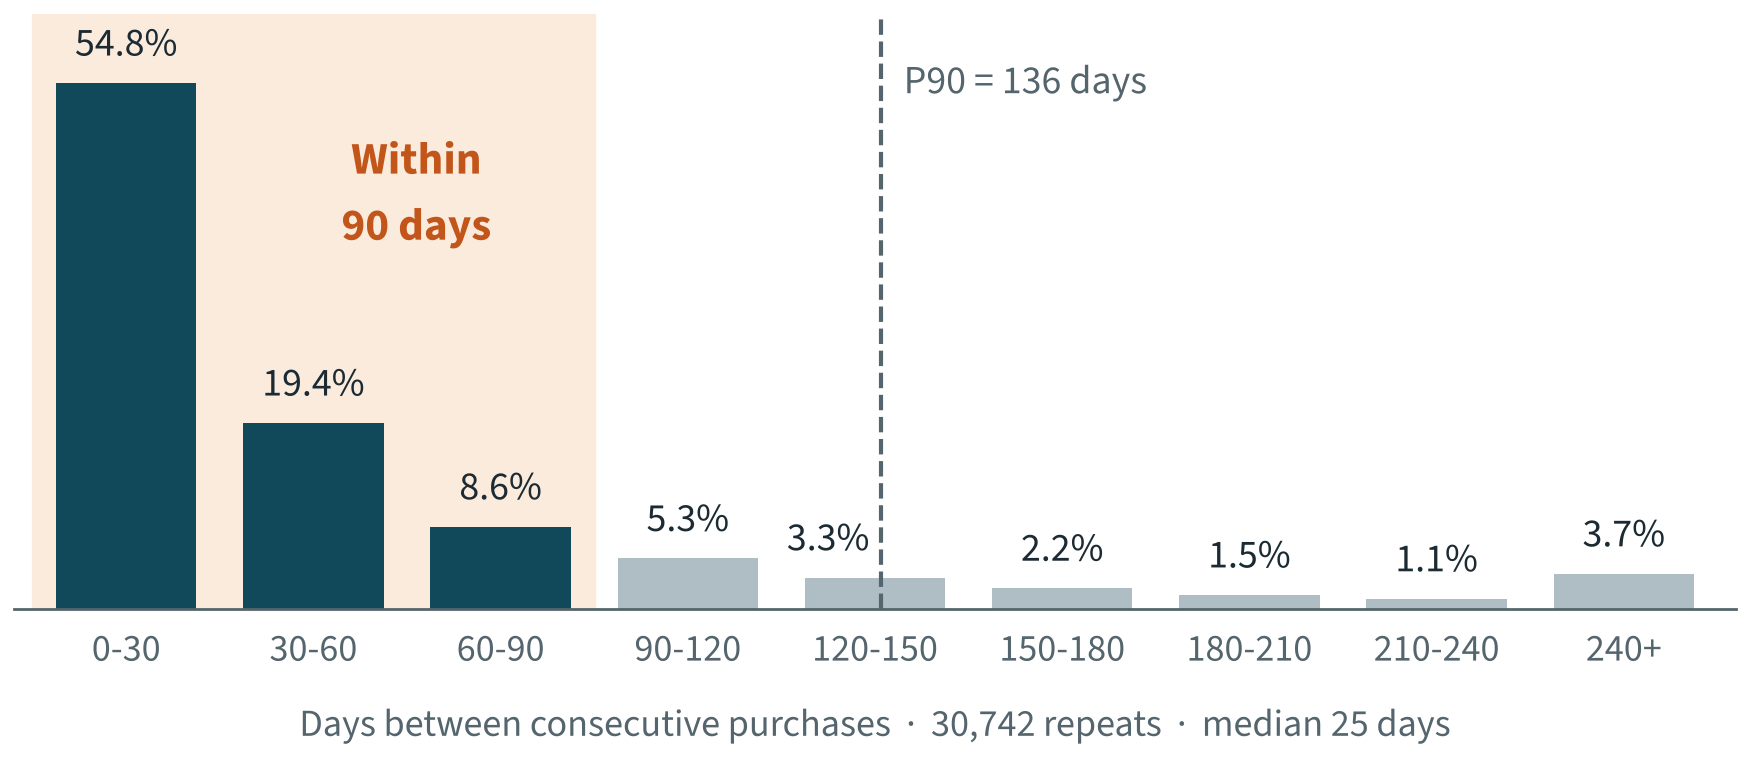
\includegraphics[width=\linewidth]{figures/repurchase_gap.png}
      \end{tcolorbox}
    \end{column}
    \begin{column}{0.46\textwidth}
      \renewcommand{\arraystretch}{1.3}
      \scriptsize
      \begin{tabular}{@{}>{\columncolor{cardgray}}p{1.25cm}%
                       >{\columncolor{cardgray}}p{2.2cm}%
                       >{\columncolor{cardgray}}p{1.7cm}@{}}
        \rowcolor{hustred}
        \color{white}\bfseries $H$ &
        \color{white}\bfseries Repeat purchases within $H$ &
        \color{white}\bfseries Training weeks left\\
        60 days  & 74.2\% & 37\\
        \rowcolor{hustgold}
        \bfseries 90 days & \bfseries 82.8\% & \bfseries 24\\
        120 days & 88.1\% & 10
      \end{tabular}\\[3pt]
      {\tiny\bfseries\color{hustred}Short $H$} {\tiny $\rightarrow$ many false churn labels. }%
      {\tiny\bfseries\color{hustred}Long $H$} {\tiny $\rightarrow$ late detection, less training data.}
    \end{column}
  \end{columns}
  \vspace{2pt}
  \begin{columns}[T]
    \begin{column}{0.31\textwidth}
      \begin{tcolorbox}[dcard, height=1.4cm]
        {\bfseries\Large\color{hustred}54.8\%}\\[-2pt]
        {\tiny\color{inkgray}of repeat purchases within 30 days: the largest bin, but not enough}
      \end{tcolorbox}
    \end{column}
    \begin{column}{0.25\textwidth}
      \begin{tcolorbox}[dcard, height=1.4cm]
        {\bfseries\Large\color{hustred}82.8\%}\\[-2pt]
        {\tiny\color{inkgray}of repeat purchases within 90 days}
      \end{tcolorbox}
    \end{column}
    \begin{column}{0.37\textwidth}
      \begin{tcolorbox}[ddark, height=1.4cm]
        {\bfseries\normalsize $R_{\max}$ = 136 days (P90)}\\[1pt]
        {\tiny No purchase for 136+ days = already gone, nothing left to predict.}
      \end{tcolorbox}
    \end{column}
  \end{columns}
  \dnext{Next: with this 90-day line, we build the RFM groups $\rightarrow$}
  \note{We define churn as no purchase within $H$ days, and we set $H$ from the
  purchase rhythm. More than half of repeat purchases happen within 30 days,
  but that cutoff would miss too many. At 60 days, one in four repeat purchases
  would arrive after we had already called the customer churned. At 120 days,
  we gain only five points but training data drops from 24 weeks to 10. So 90
  days is the balance: it covers 83\% of returns. And anyone silent for more
  than 136 days is effectively gone. (About 35 seconds)}
\end{frame}

% ============================================================
% 4. Customer groups and their value
% ============================================================
\begin{frame}[t]{4 \textperiodcentered{} Six behaviour groups; two hold 63\% of revenue}
  \vspace*{-0.55cm}
  \begin{columns}[T]
    \begin{column}{0.36\textwidth}
      \renewcommand{\arraystretch}{1.8}
      \footnotesize
      \begin{tabular}{@{\hspace{3pt}}l@{\hspace{0.45cm}}l@{\hspace{3pt}}}
        \rowcolor{hustred}
        \color{white}\bfseries Segment & \color{white}\bfseries Rule\\
        \rowcolor{cardgray}
        \color{hustred}Champions     & Top 10\% M, R $\le$ 90\\
        \rowcolor{white}
        \color{hustred}VIP at risk   & Top 10\% M, R $>$ 90\\
        \rowcolor{cardgray}
        \color{inkgray}Loyal         & R $\le$ 90, F $\ge$ 4\\
        \rowcolor{white}
        \color{inkgray}Developing    & R $\le$ 90, F = 2--3\\
        \rowcolor{cardgray}
        \color{inkgray}One-time recent & R $\le$ 90, F = 1\\
        \rowcolor{white}
        \color{inkgray}Inactive      & R $>$ 90
      \end{tabular}
    \end{column}
    \begin{column}{0.60\textwidth}
      \begin{tcolorbox}[dfig]
        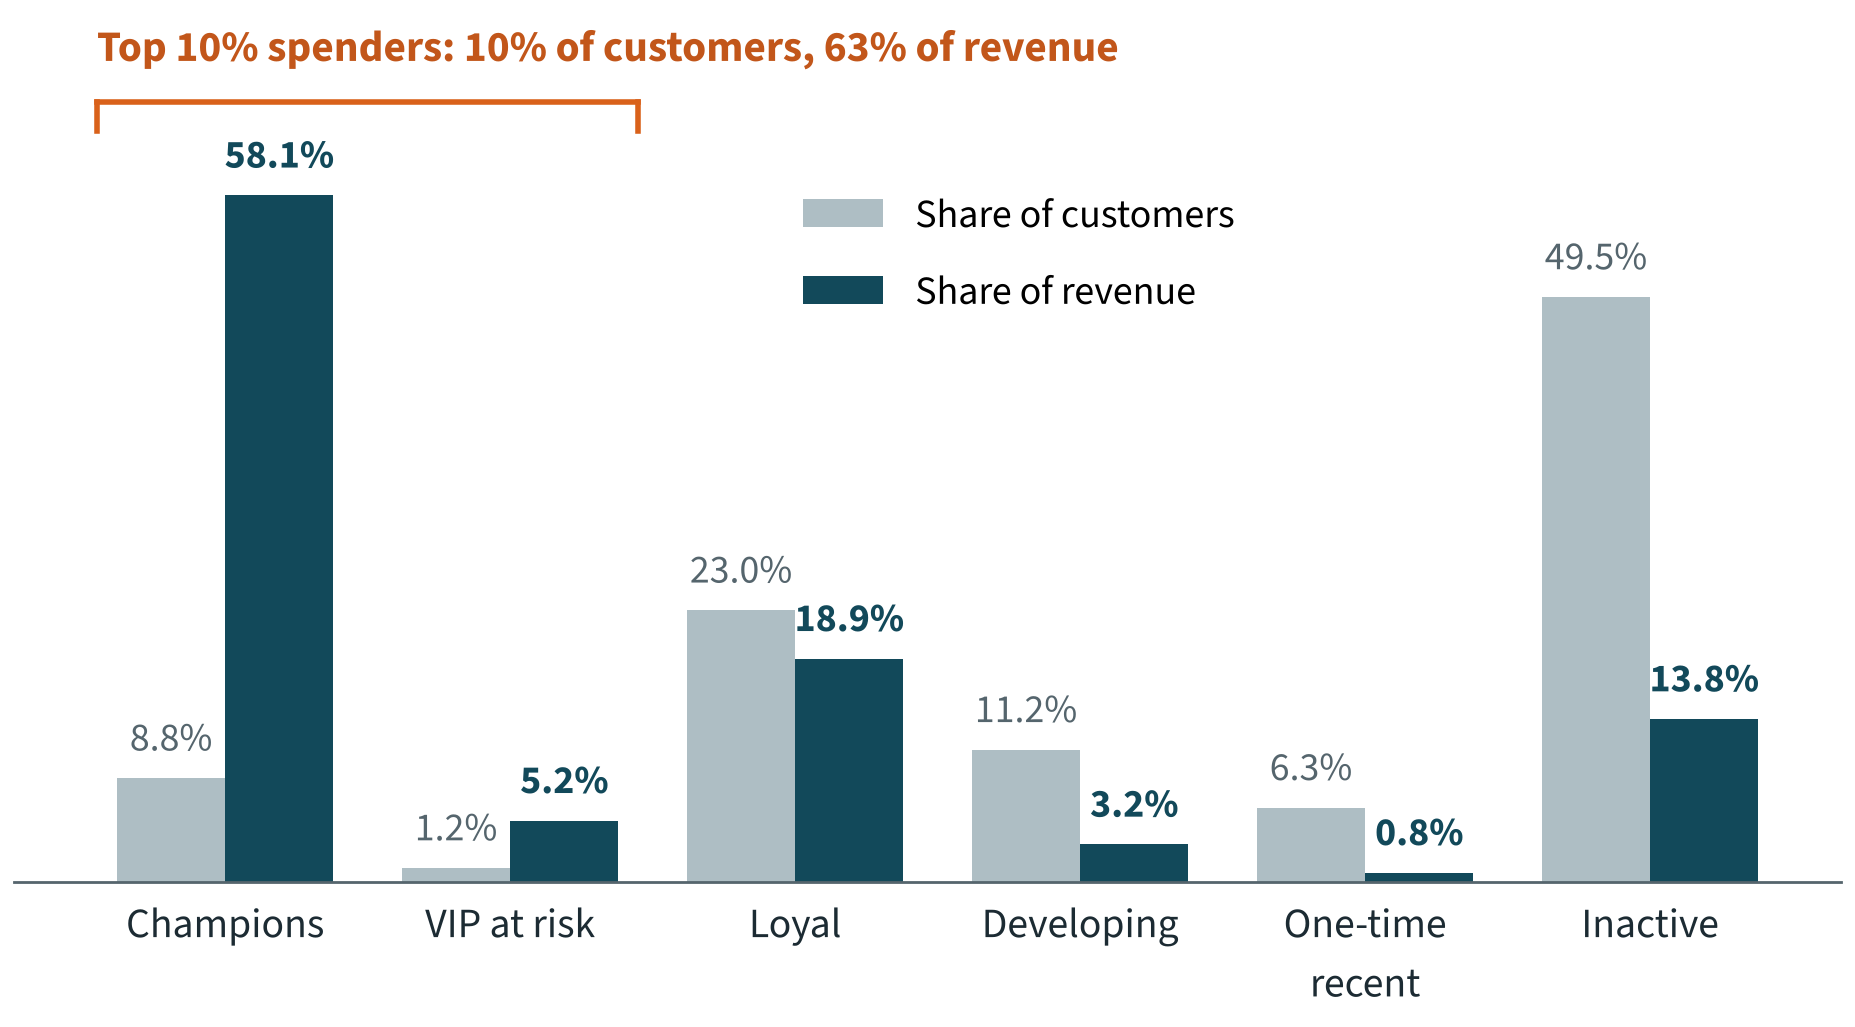
\includegraphics[width=\linewidth]{figures/rfm_segment_share.png}
      \end{tcolorbox}
    \end{column}
  \end{columns}
  \dnext{Next: predict which valuable customers won't buy in the next 90 days $\rightarrow$}
  \note{With that 90-day line and a spend threshold at the top 10\%, we built
  our RFM segments: recency tells us who is still active, frequency how
  habitual they are, and spend how valuable they are. The result is very
  concentrated: Champions and VIP at risk are only 10\% of customers but bring
  63\% of revenue. VIP at risk are exactly the high-value customers who have
  crossed the 90-day line. Meanwhile half of all customers are already inactive
  and bring only 14\%. So the next step is to predict which valuable customers
  are about to cross that line, before they do. (About 35 seconds)}
\end{frame}

\end{document}
